\documentclass[conference]{IEEEtran}
\usepackage[utf8]{inputenc}
\usepackage{cite}
\usepackage{tabularx} % Required for the table
\usepackage{array}    % Required for custom column types
\usepackage{longtable}
\usepackage{booktabs}
\usepackage{adjustbox} % To allow scaling of tables
\usepackage{caption}
\usepackage{stfloats}
\usepackage{authblk}
\usepackage{algorithm}      % For algorithm environment
\usepackage{algpseudocode}  % For algorithmicx commands

\begin{document}

\title{Power, Area and Thermal Prediction in 3D Network-on-Chip using Machine Learning}

\author{Abhijith C, Anand M K \\
Department of Computer Science and Engineering \\ 
National Institute of Technology Karnataka (NITK) \\ 
Surathkal, India\\
Email: \{abhijithc.242cs003, anandmk.242cs008\}@nitk.edu.in}

\maketitle

\section{Proposed Methodology}

Machine learning (ML) algorithms are widely used in various real-time predictions, such as energy consumption prediction and weather forecasting. The Power, Area and Temperature (PAT) prediction of Network-on-Chip can also leverage the ability of machine learning models. However, the lack of availability of a proper public dataset is a crucial issue. In addition, most existing studies focus on power, area or thermal analysis independently. Frameworks involving simultaneous analysis of all three parameters are rare in current research.

This work proposes a hybrid model that combines ML and DL algorithms. The ML component of the hybrid model uses algorithms such as linear regression and decision trees to predict area and power, which have a linear relationship with NoC parameters. The DL component of the model uses convolutional neural networks (CNNs) that learn complex nonlinear relationships in NoC to predict temperature. The algorithms can predict PAT values for unseen input NoC configuration based on their learning. The prediction of both models is combined to produce a single output in the hybrid model.

\subsection{Dataset Creation}

\begin{algorithm}
\caption{Algorithm for Proposed Framework}\label{alg:pat_prediction}
\begin{algorithmic}[1]
    \State \textbf{Input:} Set of NoC parameters: Topology, Traffic Pattern, PIR (X, Y, Z), Buffer Size, Packet Size, Sample Period
    \State \textbf{Output:} Predicted values of Power, Area, and Temperature
    
    \State \textbf{Step 1: Dataset Creation}
    \State Create dataset using simulation tool (PAT Noxim) based on input NoC parameters
    \State Extract Power, Area, and Temperature as output labels
    
    \State \textbf{Step 2: Data Preprocessing}
    \State Normalize or scale the dataset
    
    \State \textbf{Step 3: Train-Test Split}
    \State Split the dataset into Training, Validation, and Test sets (e.g., 70\% training, 15\% validation, 15\% testing)
    
    \State \textbf{Step 4: Model Training}
    \State \textbf{ML Component:}
    \State Train a \textbf{Linear Regression} model for Power and Area prediction
    \State Train a \textbf{Decision Tree} model for Power and Area prediction
    
    \State \textbf{DL Component:}
    \State Train a \textbf{CNN} for Temperature prediction
    
    \State \textbf{Step 5: Model Evaluation}
    \State Use validation data to evaluate both models
    
    \State \textbf{Step 6: Combine Predictions}
    \State Combine the outputs from the ML and DL models for final Power, Area, and Temperature predictions
    
    \State \textbf{Step 7: Testing and Final Prediction}
    \State Test the combined model on the test set and make the final prediction
    
    \State \textbf{End}
\end{algorithmic}
\end{algorithm}


\begin{figure}[h]  % Begin the figure environment
    \centering
    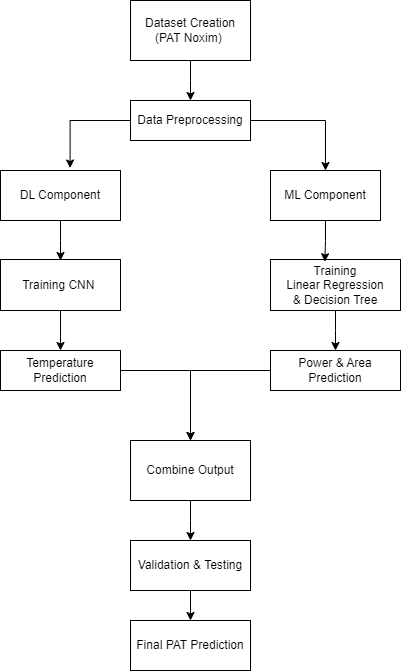
\includegraphics[width=0.8\linewidth]{Proposed.png}  % Specify the path to your image
    \caption{Illustration of the Proposed Framework}  % Add a caption for the image
    \label{fig:proposed_framework}  % Add a label for referencing the image
\end{figure}


\end{document}

\end{document}
